\chapter[Introduction]{INTRODUCTION}
\label{intro}

Isogeometric analysis, introduced by Hughes \textit{et al.}\scite{hughes05a},
is gaining popularity as an alternative to traditional finite analysis
methods.  In an isogeometric analysis the interpolation
functions use NURBS\scite{piegl97} or a variation thereof instead of
the more traditional Lagrange interpolation or other types of local polynomial
approximation.
Both rely on use of parametric interpolation to represent both
coordinates and the dependent variables.  Both also commonly use an
isoparametric interpolation to map element shapes between the parent
and global coordinate domains.
Isogeometric methods permit the use of approximations that can be $C^p$
continuous in the analysis domain.
The method is described fully in the book by Cottrell
\textit{et al.}.\scite{cottrell09a}
Additional information on isogeometric analysis may be found in
References \cite{bazilevs06a,cottrell06a,bazilevs06b,cottrell07a,zhang07a,
bazilevs08a,elguedj08a,gomez08a,hughes08a,wall08a,
evans09a,lu09a,kiendl09a,kiendl10a,bazilevs10a,echter10a,
benson10a,benson10b,benson11b,taylor11a}

\textsl{FEAP} has been adapted to permit the specification of the
analysis region using \textit{tensor product NURBS patches}.
The current implementation includes a library of elements capable of
solving problems in solid and structural mechanics.  In addition
thermal problems may also be solved. 

The description of the data to solve a thermal, solid or structural
mechanics problem utilizing \textsl{FEAP} is described in the
companion User Manual\scite{feapu}.
Many of the commands necessary to solve a problem using an
isogeometric description are the same.  However, there are some
important differences existing and 
this manual serves as a supplement to the \textsl{FEAP} User
manual.  All manuals are maintained  on-line at the web site
\begin{verbatim}
      projects.ce.berkeley.edu/feap
\end{verbatim}
and should be consulted from time-to-time to obtain any description of
new features.

\section{NURBS interpolation on a line}

Before describing how the data is prepared for an isogeometric
analysis using \textsl{FEAP} it is important to understand how
parametric interpolation is performed.  Here we discuss the basic
aspects using a one-dimensional interpolation along a line.  The basic
forms include use of a parametric description in terms of a parent
coordinate, $u$.  The parametric coordinate is used to describe a
\textit{knot vector} with $m$ values.
In the current \textsl{FEAP} implementation only
\textit{open knot vectors} are implemented (this could change in
future).  An open knot vector is described by an
increasing sequence of values. For example one may have the knot
vector with $m = 8$ values
\begin{displaymath}
\B{U} = \begin{bmatrix} 0 & 0 & 0 & 0.25 & 0.8 & 1 & 1 & 1 \end{bmatrix}
\end{displaymath}
The first an last values of an open knot vector are repeated $m$ times
and will describe a polynomial of degree $p = m -1$.  Thus the above
knot vector is capable of describing a quadratic polynomial.
Knot vectors for which the individual knots are placed at equal
intervals along the parent coordinates are called \textit{uniform knot
vectors}.  Those in which the intervals vary are called
\textit{non-uniform knot vectors}.  In
isogeometric analysis increments along the knot vector describe
individual \textit{element} intervals.  Thus the above knot vector
would describe three element intervals: $[0 ~ 0.25]$; $0.25 ~ 0.8$; and
$[0.8 ~ 1]$.  The introduction of each knot lowers the continuity of the
polynomial interpolation by \textit{one (1)}. Thus, at the location of
the knots $0.25$ and $0.8$ the continuity is reduced from two to one.
Thus, the second derivative of the (as yet undefined polynomial function)
will have a slope discontinuity at the knot points.  If an additional
knot is \textit{inserted} at $0.25$ giving the new knot vector
\begin{displaymath}
\B{U} = \begin{bmatrix} 0 & 0 & 0 & 0.25 & 0.25 & 0.8 & 1 & 1 & 1 \end{bmatrix}
\end{displaymath}
no new element interval is created (i.e., there are still only three
element intervals) but the continuity is reduced to degree 1 at $0.25$
and a slope discontinuity may now exist in the first derivative.

An polynomial function for a knot vector may be created using
B-splines\scite{piegl97}.  A B-spline may be described
starting with
\begin{displaymath}
B_{i,0}(u) = \left\{ \begin{array}{l}
1; ~~ \text{if} u_i \le u < u_{i+1} \\
0; ~~ \text{otherwise}
\end{array} \right.
\end{displaymath}
followed by the recursion
\begin{displaymath}
B_{i,p}(u) = \dfrac{u - u_i}{u_{i+p} - u_i} B_{i,p-1}(u)
+ \dfrac{u_{i+p+1} - u}{u_{i+p+1} - u_{i+1}} B_{i+1,p-1}(u)
\end{displaymath}
Note the interpolation is described in terms of the knot locations of
$\B{U}$ and each evaluation of the recursion adds one additional
function. In the recursion the ratio $0/0$ can occur and is defined
as $0$.
The basis functions $B_{i,0}$ are piecewise constants.  Thus the first
recursion will create piecewise continuous linear polynomials.

\subsubsection{Example 1:}

Consider the knot vector $\B{U} = \begin{bmatrix} 0 & 0 & 1 & 1
\end{bmatrix}$.  This has the zeroth order basis functions
\begin{displaymath}
\begin{array}{l}
N_{0,0} = 0  ~~; ~~  -\infty < u < \infty \\
N_{1,0} = \left\{
\begin{array}{l}
1 ~~; ~~ 0 \le u <  1 \\
0 ~~; ~~ \text{otherwise}
\end{array} \right.\\
N_{2,0} = 0  ; ~~  -\infty < u < \infty
\end{array}
\end{displaymath}
Applying the recursion formula gives
\begin{displaymath}
\begin{array}{l}
N_{0,1} = \dfrac{u-0}{0 - 0} N_{0,0} + \dfrac{1 - u}{1-0} N_{1,0} =
\left\{ \begin{array}{l}
1 - u ~~; ~~ 0 < u <  1 \\
0 ~~ ~~; ~~ \text{otherwise}
\end{array} \right. \\
N_{1,1} = \dfrac{u - 0}{1 - 0} N_{1,0} + \dfrac{ 1 - u}{1 - 1} N_{2,0} =
\left\{
\begin{array}{l}
u ~~; ~~ 0 < u <  1 \\
0 ~~; ~~ \text{otherwise}
\end{array} \right.
\end{array}
\end{displaymath}
These are identical to the linear Lagrange polynomials
and are only $C_0$ continuous.  The open knot vector of a
$C_0$ function has only two repeated first and last entries.
Results using such a form in an isogeometric formulation will produce
identical results to linear order Lagrange elements.  Thus
an isogeometric analysis usually implies use of quadratic an higher order
description of open knot vectors.

The interpolation of the coordinates along the line is given by
\begin{displaymath}
\B{x} = \sum_{i=1}^n B_{i,p} \, \tilde{\B{x}}_i
~~\text{where}~~ n = m - p - 1
\end{displaymath}
The parameters $\tilde{\B{x}}_i$ are called \textit{control points}
and take the place of the \textit{nodes} of a traditional finite
element analysis.  There are fundamental differences between control
points and nodes.

\subsubsection{Example 2:}

\begin{figure}[t!]
\begin{center}

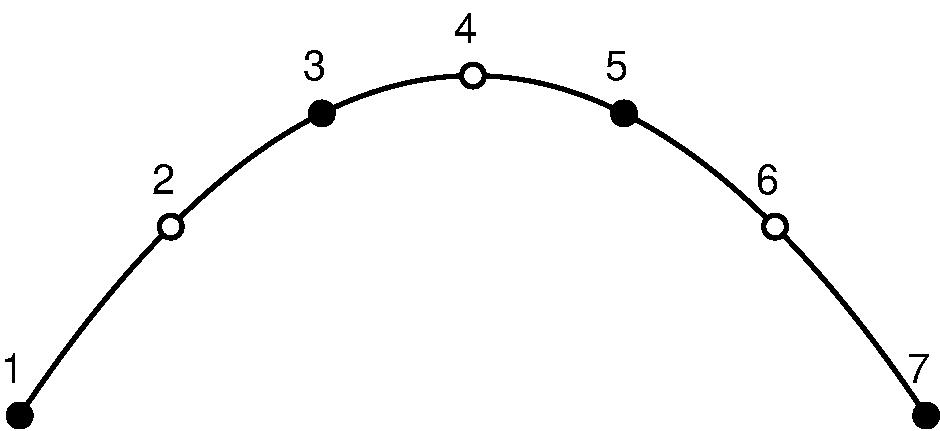
\includegraphics[width=3in]{figs/parab_3fe_L2}

\centerline{(a) Parabolic curve with 3 quadratic elements}

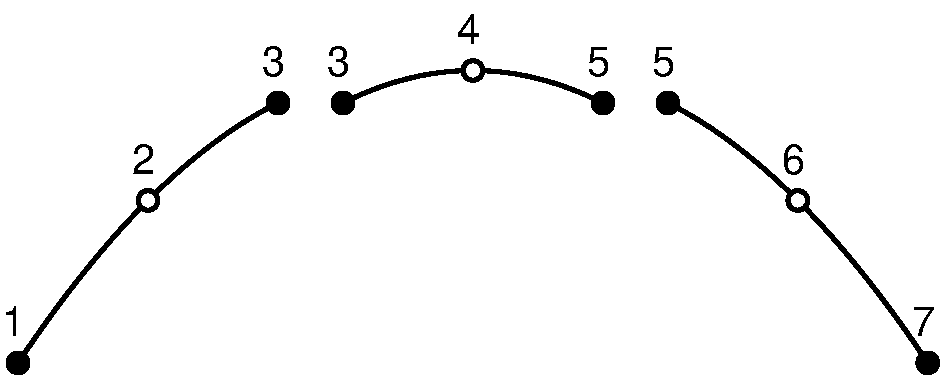
\includegraphics[width=3in]{figs/parab_3el_L2}

\centerline{(b) Split of  curve into individual elements}

\caption{Lagrange interpolation of a parabola \label{fig1l} }
\end{center}
\end{figure}

As an example let us consider the description of a parabolic line
using quadratic degree interpolation and three equal size elements in
the parametric domain.  For a standard finite element interpolation we
use the three Lagrange shape functions\scite{zt1n7}
\begin{displaymath}
\begin{split}
N_1(\xi) &= \tfrac{1}{2} (\xi^2 - \xi ) \\
N_2(\xi) &= \tfrac{1}{2} (\xi^2 + \xi ) \\
N_3(\xi) &= (1 - \xi^2)
\end{split}
\end{displaymath}
The specific parabola is defined
on the interval $-12 \le x \le 12$ which has altitude $y = 9$ at $x=0$ 
and end values $y = 0$ at $x = \pm 12$.
The location of the nodes for a Lagrange interpolation are placed at
7 points equally spaced along the $x$-axis with values
\begin{displaymath}
\begin{split}
\tilde{\B{x}}_1 &= \begin{Bmatrix} -12 \\ ~~0 \end{Bmatrix}  ~~;~~
\tilde{\B{x}}_2 = \begin{Bmatrix} -8 \\ ~5 \end{Bmatrix}  ~~;~~
\tilde{\B{x}}_3 = \begin{Bmatrix} -4 \\ ~8 \end{Bmatrix}  ~~;~~
\tilde{\B{x}}_4 = \begin{Bmatrix} 0 \\ 9 \end{Bmatrix}  \\
\tilde{\B{x}}_5 &= \begin{Bmatrix} 4 \\ 8 \end{Bmatrix}  ~~;~~
\tilde{\B{x}}_6 = \begin{Bmatrix} 8 \\ 5 \end{Bmatrix}  ~~;~~
\tilde{\B{x}}_7 = \begin{Bmatrix} 12 \\ ~0 \end{Bmatrix}
\end{split}
\end{displaymath}
A plot of the line using the Lagrange interpolation is shown in Fig.
\ref{fig1l}.  The $C_0$ nodes are shown as black dots and the
internal nodes for $N_3$ by white dots.
In the (b) part of the figure we show the individual elements and
their associated nodes.

\begin{figure}[t!]
\begin{center}

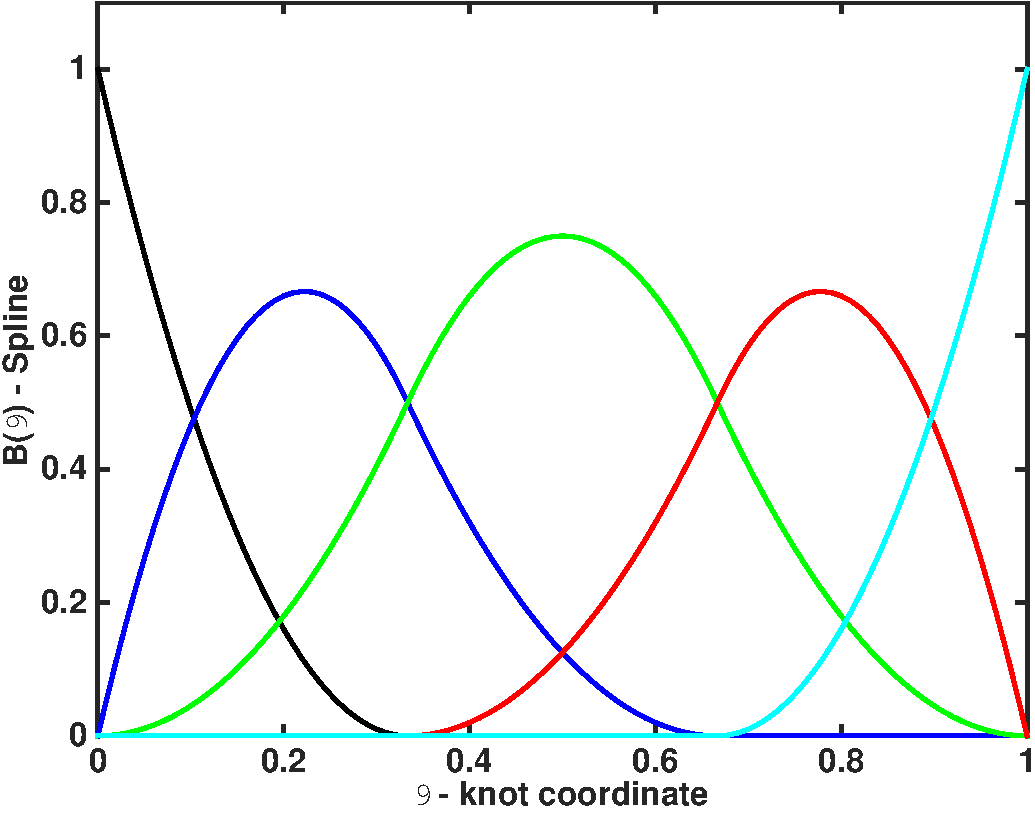
\includegraphics[width=3.5in]{figs/bspline_2_5}

\caption{Quadratic B-spline for quadratic knot with three elements. Generates
5-functions. \label{fig1b} }
\end{center}
\end{figure}


\begin{figure}[b!]
\begin{center}

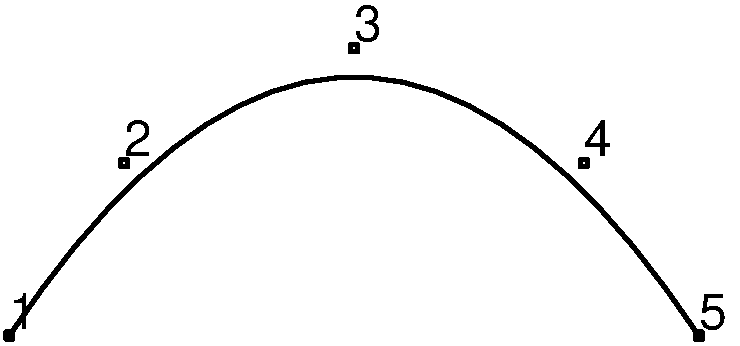
\includegraphics[width=3.5in]{figs/bspline_xy_5}

\centerline{(a) Quadratic B-spline curve with 5 control point
positions.}

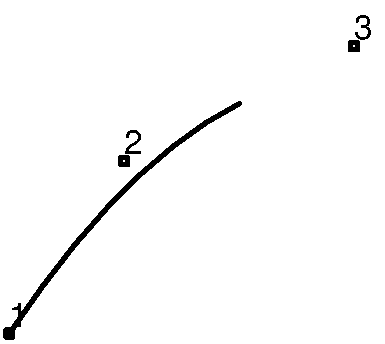
\includegraphics[width=1.5in]{figs/belm_1}
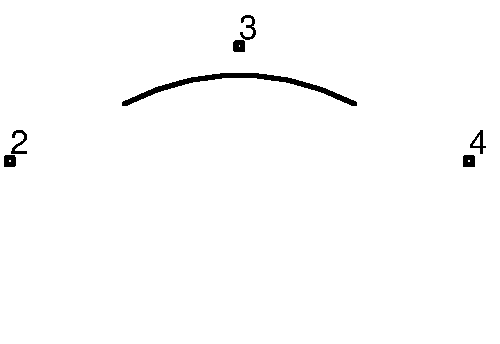
\includegraphics[width=2.0in]{figs/belm_2}
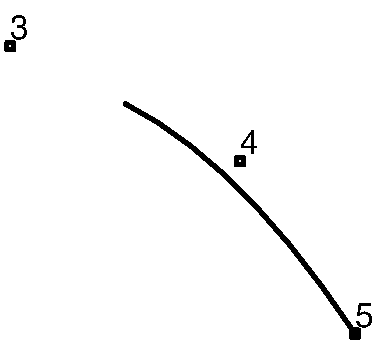
\includegraphics[width=1.5in]{figs/belm_3}

\centerline{(b) Quadratic B-spline elements.}

\caption{B-spline curve for parabola.  \label{fig1bel} }

\end{center}
\end{figure}

Next we consider the same parabola where the interpolation is
performed using quadratic B-spline interpolation.  To create three
elements we use the knot vector
\begin{displaymath}
\B{U} = \begin{bmatrix} 0 & 0 & 0 & \tfrac{1}{3} & \tfrac{2}{3} & 1 & 1 & 1 \end{bmatrix}
\end{displaymath}
Applying the recursion formula generates creates only 5 unique
functions as shown in Fig. \ref{fig1b}.
The location of the control points to construct the desired parabola
are located at
\begin{displaymath}
\tilde{\B{x}}_1 = \begin{Bmatrix} -12 \\ ~~0 \end{Bmatrix}  ~~;~~
\tilde{\B{x}}_2 = \begin{Bmatrix} -8 \\ ~6 \end{Bmatrix}  ~~;~~
\tilde{\B{x}}_3 = \begin{Bmatrix} -0 \\ 10 \end{Bmatrix}  ~~;~~
\tilde{\B{x}}_4 = \begin{Bmatrix} 8 \\ 6 \end{Bmatrix}  ~~;~~ 
\tilde{\B{x}}_5 = \begin{Bmatrix} 12 \\ 0 \end{Bmatrix}
\end{displaymath}
These produce the parabola shown in Fig. \ref{fig1bel}.

There are distinct differences between B-spline interpolation and
Lagrange interpolation.  Except for the end points of an open knot
the control points do not lie on the curve of the parabola. Moreover,
the description of each element involves control points that overlap
between elements -- this is what allows for the increased continuity.
Last, we observe that the B-spline functions are positive everywhere. 
The sum of all the B-splines of a order $p$ always equals one, thus
B-splines are a \textit{partition of unity}.
There are other aspects related to the use of spline interpolation,
these are discussed in the references cited above.

\subsection{NURBS functions and B\'{e}zier extraction}

Non-uniform rational B-splines (or simply NURBS) utilize an additional
parameter to describe the control point -- these are positive weights $w_i$.
The NURBS functions are defined as
\begin{displaymath}
N_{i,p}(u) = \dfrac{B_{i,p}(u) w_i}{\sum_{j=1}^n B_{j,p}(u) w_j}
\end{displaymath}
Use of the weights allows for shapes of different types, including
circular arcs.  If all the weights are unity, the denominator sums to
one and B-splines are recovered.

The construction of the B-spline functions using the recursion
formula is awkward and can become time consuming for high-degree
functions.  An alternative is to use B\'{e}zier extraction to relate
the B-spline functions in each non-zero knot interval to Bernstein
polynomials. This is described in detail by Borden \textit{et
al.}\scite{borden11a}.  For each knot interval a $p+1 \times p+1$
matrix $\B{C}^e$ may be described such that
\begin{displaymath}
B_{i,p}(\xi) = {C}_{ij}^e b_{j,p}(\xi) 
\end{displaymath}
where the $b_{j,p}$ are Bernstein polynomials.  For quadratic
polynomials on the element interval $-1 \le \xi \le 1$ the Bernstein
polynomials are
\begin{displaymath}
\begin{split}
b_{1,2} &= \tfrac{1}{4} ( 1 - \xi)^2 \\
b_{2,2} &= \tfrac{1}{4} ( 1 + \xi)^2 \\
b_{3,2} &= \tfrac{1}{2} ( 1 - \xi^2)
\end{split}
\end{displaymath}
Use of B\'{e}zier extraction greatly simplifies the construction of
shape functions once the \textit{extraction matrices} $\B{C}^e$ are known.  
The extraction matrices are defined by a simple \textit{knot insertion}
algorithm as described in Piegl \& Tiller\scite{piegl97}.

Higher dimensional interpolation may be defined by taking products of
the one-dimensional form in each desired coordinate direction.  These
are called \textit{tensor product} forms and currently form the basis
for nearly all the developments currently available in \textsl{FEAP}.

With this brief set of preliminaries, we now describe how the data is
prepared for a NURBS based solution using \textsl{FEAP}.

\chapter{\texttt{NURBS} mesh description}
\label{nmesh}

We describe how to define a tensor product NURBS patch for a
\textsl{FEAP} analysis.  Tensor product patches may be described for
one, two or three dimensional applications.

\section{Control information: Start of problem}
\label{ncontrol}

The start of an analysis begins with the standard \textsl{FEAP} control
information. However, for some element forms special care is needed in
setting the number of degrees of freedom (\texttt{NDF}).  The
the control data consists of two lines:
\begin{verbatim}
       FEAP * * <any description of the problem>
         NUMCP NUMEL NUMMAT NDM NDF NEN
\end{verbatim}
where
\begin{verbatim}
       NUMCP  = Number of control points
       NUMEL  = Number of elements
       NUMMAT = Number of material sets
       NDM    = Mesh spatial dimension
       NDF    = Maximum number of degrees of freedom/control point
       NEN    = Maximum number of control points on an element
\end{verbatim}
Using the data preparation approach described below for
an isoparametric analysis the number of control points
(\texttt{NUMCP}), elements (\texttt{NUMEL}) and size of an element
(\texttt{NEN}) are generally not
known at the start of an analysis.  This is due to the specified order
of elevation of the knot vector and/or the number of inserted knots;
each of which are operations that may be performed using \textsl{FEAP} command
instructions described in later sections of this report.  Accordingly,
these values should be set to zero, \textsl{FEAP} will assign values
as the mesh for the problem is constructed.

For solution of problems using the displacement form of \textit{solid}
elements the value of \texttt{NDM = NDF} (or more).  For \textit{thermal}
analyses the values of \texttt{NDM} is the spatial dimension of the
problem  and \texttt{NDF = 1} (or more).  These are identical to the
usual finite element analysis values as
described in the \textsl{FEAP} User manual\scite{feapu}.

For \texttt{MIXED} solid elements (those based on a
$\B{u}$-$p$-$\theta$ formulation as described in references
\cite{zt1n7} and \cite{taylor11a}) the value of \texttt{NDF} must be
set to \texttt{NDM+1}.  Thus for a three dimensional analysis using the
mixed solid elements the control data is input as
\begin{verbatim}
       FEAP * * <title information for mixed analysis>
         0 0 0 3 4 0
\end{verbatim}

For analyses using the Kirchhoff-Love thin element the parameters are
set as $NDM = 3$ and $NDF = 3$ or more.
Thus for the shell the control records are set as
\begin{verbatim}
       FEAP * * <title information for shell analysis>
         0 0 0 3 3 0
\end{verbatim}
Note it is not necessary to provide the number of nodes, elements, material sets
or nodes/element.  These will be determined based on the subsequent input
data provided.

Alternatively, the above statements now may be given for the mixed
solid as
\begin{verbatim}
       FEAP * * <title information for mixed solid analysis>
         ndm = 3 
         ndf = 4
\end{verbatim}
and for the shell as
\begin{verbatim}
       FEAP * * <title information for shell analysis>
         ndm = 3 
         ndf = 3
         nad = 2
\end{verbatim}
If the solid is encased in a shell the parameters are given as
\begin{verbatim}
       FEAP * * <title information for solid & shell analysis>
         ndm = 3 
         ndf = 4
         nad = 2
\end{verbatim}

\section{MATERIAL set description}
\label{nmaterial}

The specification of material properties generally follows the
descriptions described in the \textsl{FEAP} User Manual\scite{feapu}.
The types of elements available are:
\begin{verbatim}
       SOLId           - Solid DISPlacement or MIXEd types
       THERmal         - Fourier heat conduction 
       NURB_THIN_SHELL - Kirchhoff-Love thin shell
       NURB_SLOPE      - Slope enforcement for K-L shell
       PRESsure        - Pressure or traction loading on surface
       USER enum
\end{verbatim}
Note that the required specification for the element type must include
all the letters given in upper case above.

A NURBS solution may be
used for both small and large displacement solid elements of type
\texttt{DISPlacement} or \texttt{MIXEd} only.  The thin
Kirchhoff-Love shell formulation 
is specified by \texttt{NURB\_THIN\_SHELL} for both the large and small displacement
formulation.

\subsection{Activation of NURBS interpolations}

Activation of the NURBS option is given during the
specification of the \texttt{MATErial} property data by including the
statement
\begin{verbatim}
       NURBs interpolation q1 q2 q3
\end{verbatim}
as part of the data specification.
The parameters \texttt{q1}, \texttt{q2}, \texttt{q3} denote quadrature order
in each direction of the tensor product patch.  For two dimensional problems
it is not necessary to specify \texttt{q3}.

\subsection{SOLId element material sets}

To solve a problem using \texttt{SOLId} type elements the material
data set is given as:
\begin{verbatim}
       MATErial ma
         SOLId
           <ELAStic, PLAStic, VISCoelastic, etc. material model>
           NURBs <option> q1 q2 q3
            ! Blank end record
\end{verbatim}
Currently, the \texttt{option} parameter is not used.  In future it
will be used to specify the type of interpolation form
(\textit{T-spline}, etc.).
The values of \texttt{q1}, \texttt{q2} and \texttt{q3} are the number of
quadrature points in the 1,2 and 3 directions (currently, between 1 and 5).

Specific forms of data for constitutive models, body forces, etc. are described
in the \textsl{FEAP} User Manual.\scite{feapu}

\subsection{THERmal element material sets}

To solve a problem using the \texttt{THERmal} type elements the
material data set is given as:
\begin{verbatim}
       MATErial ma
         THERmal
           FOURier <isotrop, orthotropic ...>
           <additional data such as DENSity ...>
           NURBs <option> q1 q2 q3
            ! Blank end record
\end{verbatim}
The values of \texttt{q1}, \texttt{q2} and \texttt{q3} are the number of
quadrature points in the 1,2 and 3 directions (currently, between 1 and 5).

Description of the material models, etc. is again in the \textsl{FEAP}
User Manual.

\subsection{NURB\_THIN\_SHELL element material sets}

To solve a problem using Kirchhoff-Love thin shell type elements the
material data set is given as:
\begin{verbatim}
       MATErial ma
         NURB_THIN_SHELL
           <ELAStic, PLAStic, VISCoelastic, etc. material model>
           THICkness SHELL h
           NURBs <option> q1 q2 q3
           <FINIte, SMALl>
            ! Blank end record
\end{verbatim}
Here the values of \texttt{q1} and \texttt{q2} are the number of
quadrature points in the 1 and 2 directions of the surface patch
describing the element (currently, between 1 and 5).
The value of \texttt{q3} is the number of
quadrature points in the shell thickness direction and must be 2 or
more.
The commands \texttt{FINIte} and \texttt{SMALl} are used to denote
the large displacement and small displacement forms, respectively.
However, if the material model applies only to finite deformation, for 
example
\begin{verbatim}
       ELAStic NEOHook E_mod nu
\end{verbatim}
then the \texttt{FINIte} is automatically selected.

Descriptions for the material models, body loading, etc. are again in
the \textsl{FEAP} User Manual (e.g., see Chapter 7 for material model
types available).

\subsection{NURB\_SLOPE element material sets}

The constraint of slope between NURBS patches is enforced by the user
element \texttt{ELMT27} and is accessed using the material set commands
\begin{verbatim}
       MATErial ma
         NURB_SLOPE
           PENAlty,,pen_value
           QUADrature <NODE, NODAl, GAUSs>
            ! Blank end record
\end{verbatim}
The number of quadrature points for all forms is 2. 
In addition, the number of degree-of-freedoms at a node must be increase to 4
in order to provide storage for the constraint forces.
The constraint maintains the initial angle defined by the two patches
during the entire solution based on control points only that define
a 6-node constraint element.  Note, the slope enforcement involves a non-linear
relation, thus, a non-linear solution method is required using, for
example
\begin{verbatim}
       LOOP,,20 ! or some number
         TANG,<LINE>,1
       NEXT
\end{verbatim}

\subsection{PRESsure: Dead and Follower loads}
\label{pressure}

The \textit{pressure load element} is specified by material set records:
\begin{verbatim}
       MATErial ma
         PRESsure
           LOAD p prop-ld
           NURBs quadr q1 q2
          <PLOT,NOPLot> !  PLOT/NOPLot surface: Default NOPLot
          <PLANe,AXISym> ! 2-d types: Default PLANe
          <DEAD,FOLLower>! Default DEAD
             ...
\end{verbatim}
Loading is specified by options \texttt{LOAD} and, for follower loads by
\texttt{FINI}te or \texttt{FOLL}ower.  Loading intensity may be associated
with the proportional loading number \texttt{prop-ld}.
The \texttt{NURBs} option specifies the quadrature order to use in the two
surface directions of a 3-d problem. For 2-d problems the second value is
not used since the surface has only one-dimension.

\subsection{USER element material sets}

User elements are also provided but vary with specific releases.
The basic input form is
\begin{verbatim}
       MATErial ma
         USER   e_num
           <user element data>
            ! Blank end record
\end{verbatim}
The \texttt{e\_num} parameter is the number of the specific user
element used.  That is if \texttt{ELMT04.f} is used then \texttt{e\_num = 4}.

A number of user elements have been
added as described in Table \ref{tab2iga}.


\begin{table}[t]
\begin{center}
\begin{tabular}{| r | p{11cm}|} \hline
\texttt{ELMT} & Description \\ \hline
 1~ & NURBS Euler-Bernoulli beam \\
 2~ & NURBS 1-d rod. \\
 3~ & NURBS 1-d displacement boundary condition \\ 
 5~ & NURBS \& T-spline thin $C^1$ plate \\
 6~ & NURBS \& T-spline thin membrane \\
20~ & Follower couple to load thin shell element \\
24~ & NURB\_THIN\_SHELL - Kirchhoff-Love shell \\
37~ & NURB\_SLOPE - Slope compatibility enforcement \\ \hline
\end{tabular}
\caption{User elements for NURBS/T-spline solutions. \label{tab2iga} }
\end{center}
\end{table}

  
\section{NURBS patch input}

Tensor product
NURBS patches are defined by specifying the \textit{control point} data using
the \texttt{NURB} command; the \textit{knot vector} in each direction
using the \texttt{KNOT} command; and  the \texttt{NPATch} command which
includes a list of control points to define the patch.
Descriptions for specifying a patch for a line, surface or solid is
described below.

Alternatively, the patch may be defined using the \texttt{NBLOck} command
and the \texttt{NSIDe} command as described in Appendix \ref{appxa}.
Descriptions for specifying each of these data types is provided below.

A NURBS patch may be specified using the minimum number of control points,
order of knot vectors and sides necessary to describe the exact geometry. 
This description may be subsequently refined by raising the order of the knot
vectors (\textit{knot elevation}) and specifying additional knot points
(\textit{knot insertion}) necessary to produce an accurate
answer (this is commonly called a \textit{k-refinement}).

\subsection{\texttt{NURBS} control point specification}

The control points for a patch are described by the \texttt{NURBs} data.  Input
of the control points uses the same command structure as for input of
\texttt{COORdinate} data with added need to specify the \textit{weight} for
the control point.  Data sets are input as:
\begin{verbatim}
       NURBs
         n1  ng1  (x(i,n1),i = 1,ndim) w(n1)
         n2  ng2  (x(i,n2),i = 1,ndim) w(n2)
          ....
          ! terminate with blank record
\end{verbatim}
where \texttt{ndim} is the mesh spatial dimension and \texttt{ng1}, \texttt{ng2}
are increments to the control point numbers.  For example, the two pairs
shown above will generate the sequence of control points
\begin{verbatim}
    n1,  n1+ng1, n1+2*ng1, ..... , n2
\end{verbatim}
with values for coordinates and weights linearly interpolated between the
two specified values.

\subsection{\texttt{KNOT} vector specification}

Currently four types of knot vectors may be used to construct NURBS patches:
CLAMped (open) knot vectors; UNCLamped knot vectors; LCLAmped knot
vector which is clamped at the start values and unclamped at the end value; and
RCLAmped which is unclmaped at the start value and clamped at the end
value.  Clamped (open) knot vectors are interpolatory at an end 
control point
whereas unclamped knot vectors are not interpolatory unless the knot vector
is repeated to give a $C_0$ point. However, unclamped knot vectors may
be used to create closed surfaces or to maintain 
greater than $C_0$ continuity between patches.

\subsubsection{CLAMped (OPEN) knot vectors}

Open knot vectors are specified by the records:\footnote{A clamped knot
may also be specified by the type OPEN.}
\setlength{\baselineskip}{12pt}
\begin{verbatim}
       KNOTs
         CLAMp n1 lknot1 (vk1(i),i=1,lknot1)
         CLAMp n2 lknot2 (vk2(i),i=1,lknot2)
          ....
           ! terminate with blank record
\end{verbatim}
\setlength{\baselineskip}{14pt}
where \texttt{n1} is the knot number, \texttt{lknot1} is the length of
the knot vector and \texttt{vk1(i)} is the list of open knot values.
Recall that only 16 items can appear on any record, thus, if the knot vector has more than 13 data entries the next 16 appear on the following line, etc.
until all the values are provided.  Open
knot vectors must begin and end with repeated values of one more than the
order of the knot.  An example for two quadratic knot vectors is
\setlength{\baselineskip}{12pt}
\begin{verbatim}
      CLAMp 1 6 0.0 0.0 0.0 3.0 3.0 3.0
      CLAMp 2 7 0.0 0.0 0.0 0.5 1.0 1.0 1.0
\end{verbatim}
\setlength{\baselineskip}{14pt}
Generally, one may start the knot at $0.0$ and go to any end value desired.  
However, the knot values \textit{must} appear in ascending order.

The specification of real values for \textsl{FEAP} do not need to
include the decimal point.  Thus, the above knot vectors may also be
given in the simpler form
\setlength{\baselineskip}{12pt}
\begin{verbatim}
      CLAMp 1 6  0 0 0 3 3 3
      CLAMp 2 7  0 0 0 0.5 1 1 1
\end{verbatim}
\setlength{\baselineskip}{14pt}

\subsubsection{UNCLamped (periodic) knot vectors}

An unclamped knot vector is specified in \textsl{FEAP} using the input form
\setlength{\baselineskip}{12pt}
\begin{verbatim}
       KNOTs
         UNCLamp n1 lknot1 order1 (vk1(i),i=1,lknot1)
         UNCLamp n2 lknot2 order2 (vk2(i),i=1,lknot2)
          ....
           ! terminate with blank record
\end{verbatim}
\setlength{\baselineskip}{14pt}
Similarly the mixed types may be specified as
\setlength{\baselineskip}{12pt}
\begin{verbatim}
       KNOTs
         LCLAmp n1 lknot1 order1 (vk1(i),i=1,lknot1)
         RCLAmp n2 lknot2 order2 (vk2(i),i=1,lknot1)
\end{verbatim}
\setlength{\baselineskip}{14pt}
For an \texttt{LCLAmp} type the initial values of the \texttt{vk1(i)} array
must be repeated for \texttt{i=1, order1+1} times; and vice versa for the
\texttt{RCLAmp} type (the last \texttt{order2} of the \texttt{vk2(i)} array
must have the same value).

It is also possible to mix types within the same \texttt{KNOTs} group
(i.e., some may be \texttt{open} while others are \texttt{uncl}).
Note that an extra field is required to set the order since knot vector
values are not repeated at the beginning and end of the \texttt{vk1(i)}
sequence.  An unclamped knot vector may be used to create a closed
surface with $C_p$ continuity (where $p$ is one less than the order)
by setting the coordinates of the start and end \texttt{order} control points
to the same value. For this case the beginning and ending overlapped knot
spacings must be the same.

In general the \texttt{UNCLamped}, \texttt{LCLAmp} and \texttt{RCLAmp} types
in \textsl{FEAP} can not create conic sections.  

\begin{figure}[!b]
\begin{center}

\centerline{
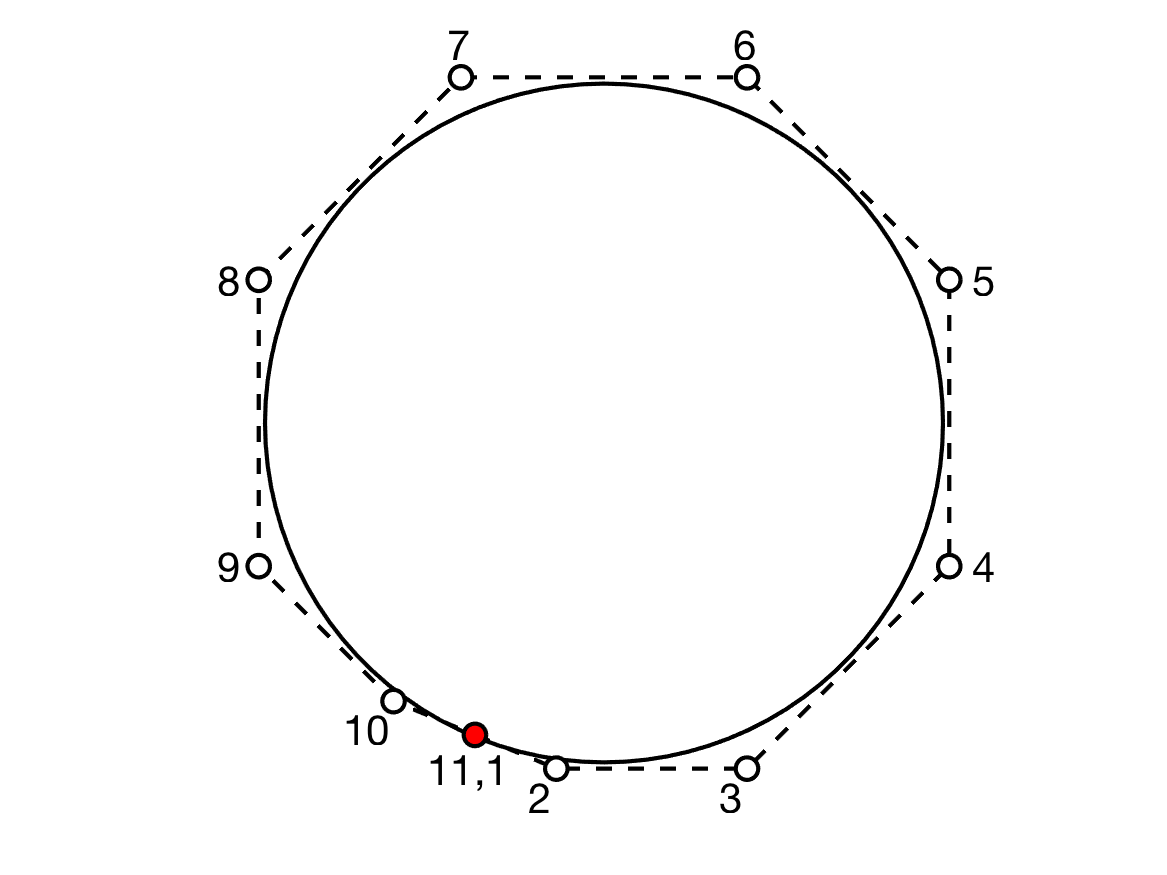
\includegraphics[height=2.75in]{figs/close_cl_8}
\hspace{0.4in}
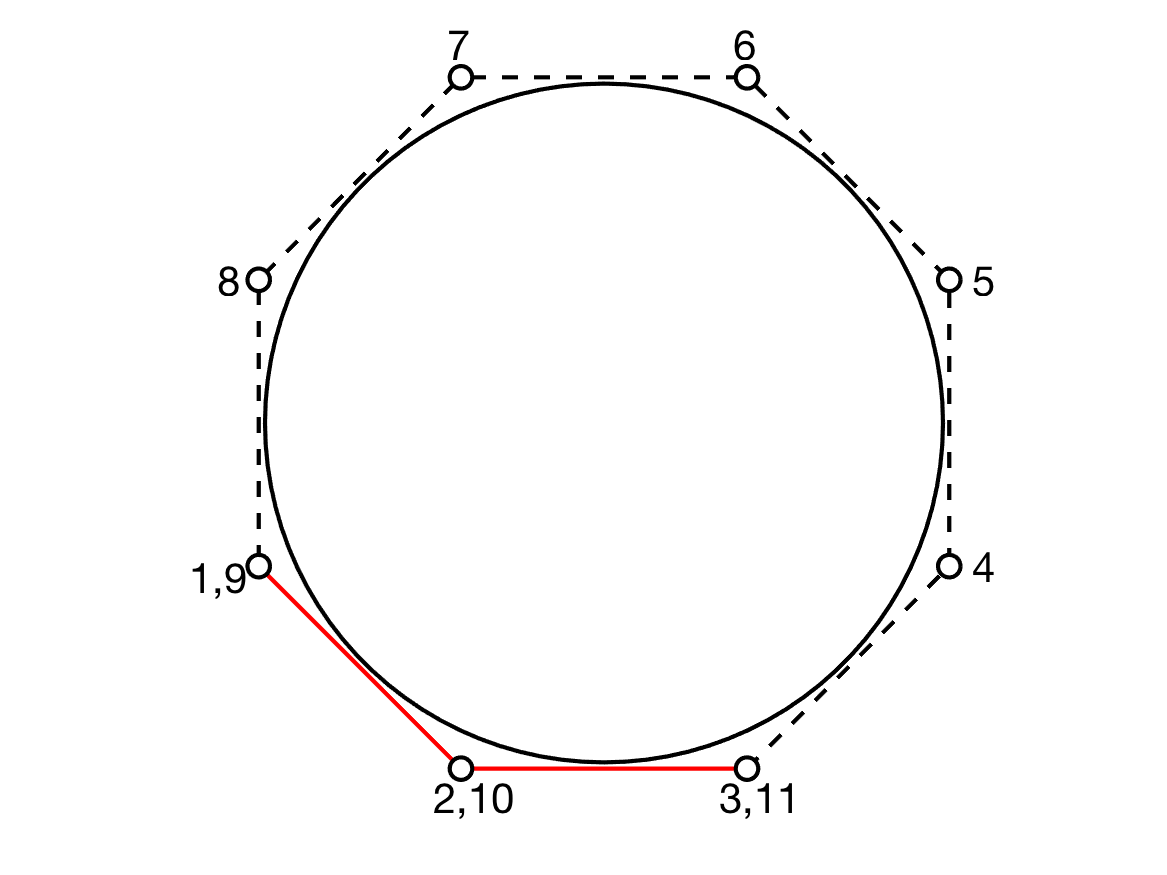
\includegraphics[height=2.75in]{figs/close_un_8}
}

\centerline{(a) Clamped knot \hspace{2in} (b) Unclamped knot}

\caption{Close ring using clamped and unclamped knot vector.  
The \textit{red} control point of (a) is $C_0$ and the \textit{red} overlap
of (b) maintains the $C_2$ continuity of the cubic curve. \label{fig2cl} }
\end{center}
\end{figure}

\begin{figure}[!t]
\begin{center}

\centerline{
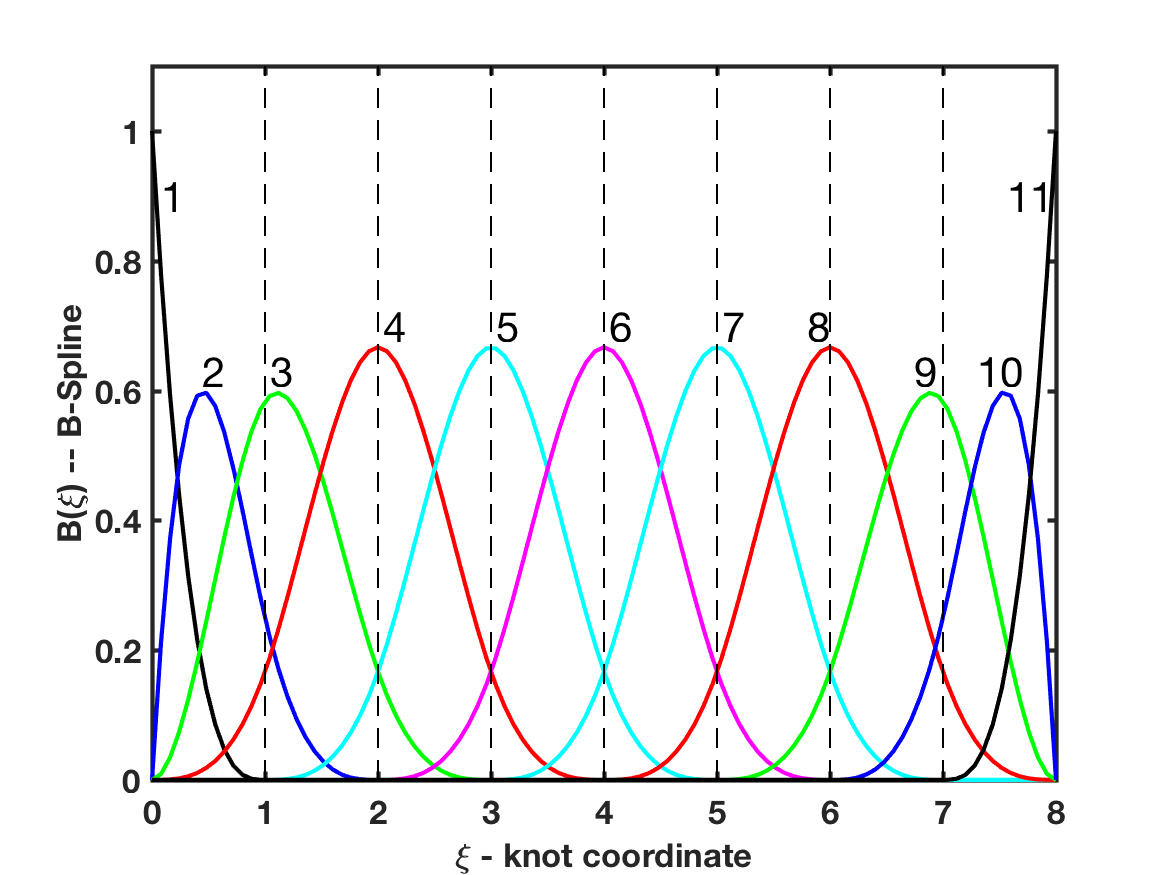
\includegraphics[width=3.00in]{figs/nurb3_1d_cl}
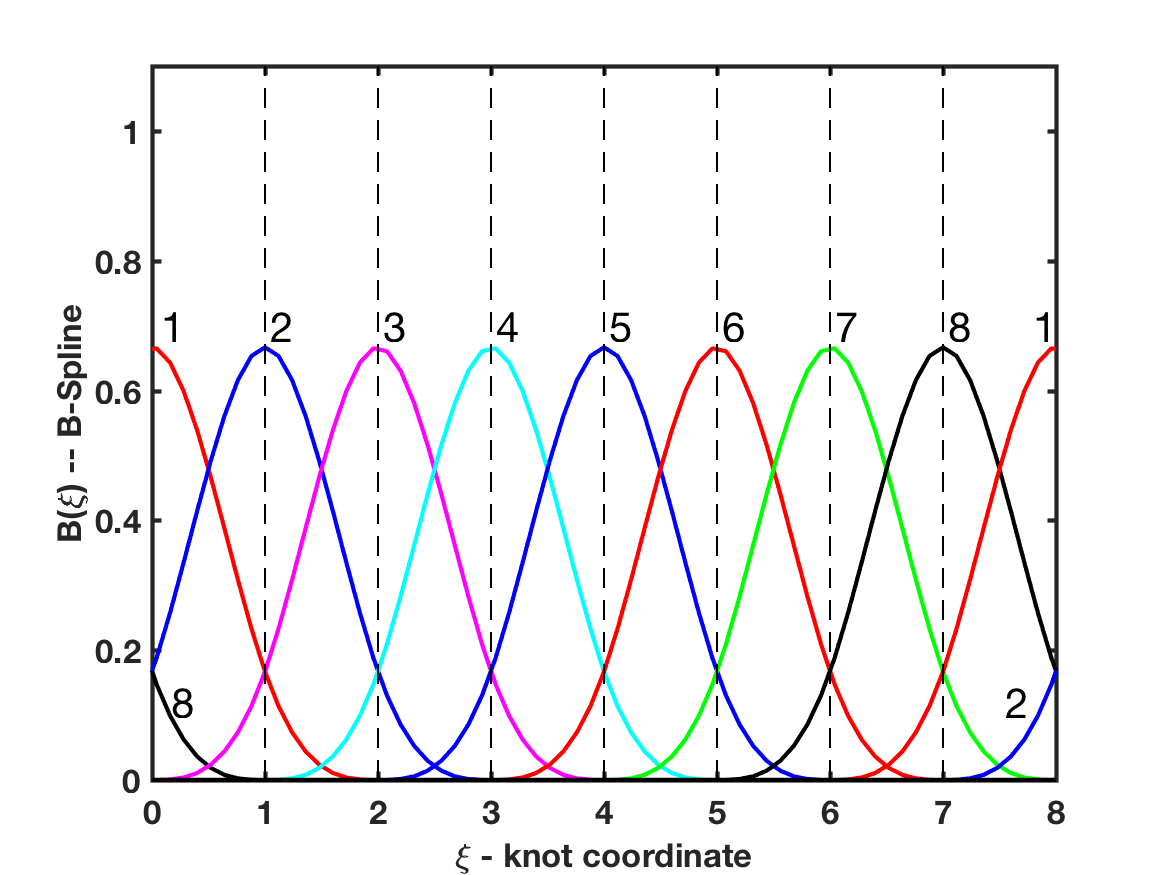
\includegraphics[width=3.00in]{figs/nurb3_1d_un}
}

\centerline{(a) Clamped B-splines \hspace{2in} (b) Unclamped B-splines}

\caption{Close ring B-splines for clamped and unclamped knot vector.  
\label{fig2b_s} }
\end{center}
\end{figure}

To close a surface using unclamped knots it is necessary to start with
uniform knot spacing and \textit{overlap} the last \texttt{order1} control
points -- that is they must have the same coordinate values.  To merge
(join) the control points of the mesh to have the same node number,
the standard
\begin{verbatim}
       TIE
\end{verbatim}
command is used (see User Manual for details\scite{feapu}).
\textit{Always use a graphical check for the mesh input to ensure that
surfaces actually are closed}.

\begin{quote}
\noindent
\textbf{Example: Closed ring}
To illustrate the use of clamped and unclamped knows in creating a closed
ring we consider the shapes shown inf Fig. \ref{fig2cl}.  The left figure
shows the control polygon and ring (which is a not a perfect circle since all
the control weights are unity). The red marked control point is a location that
can only be $C_0$ (after a \texttt{TIE}).  The right figure shows the same
ring using an \textit{unclamped knot vector}.  The red marked portion denotes
control points that are over-lapped to preserve the continuity (again after
a \texttt{TIE}).
Figure \ref{fig2b_s} shows the spline functions for each of clamped
and unclamped knots.  There are eleven (11) functions for each form, however,
due to the overlap of the control points three (3) of the functions are in
fact continuations as the number indicate.
The data for the clamped knot and control points is given
by:
\setlength{\baselineskip}{12pt}
\begin{verbatim}
       NURBs
         1 0 -4.5949E+01 -1.1093E+02 1.0000E+00
         2 0  1.6973E+01 -1.2293E+02 1.0000E+00
         3 0  5.0920E+01 -1.2293E+02 1.0000E+00
         4 0  1.2293E+02 -5.0920E+01 1.0000E+00
         5 0  1.2293E+02  5.0920E+01 1.0000E+00
         6 0  5.0920E+01  1.2293E+02 1.0000E+00
         7 0 -5.0920E+01  1.2293E+02 1.0000E+00
         8 0 -1.2293E+02  5.0920E+01 1.0000E+00
         9 0 -1.2293E+02 -5.0920E+01 1.0000E+00
        10 0 -7.4925E+01 -9.8929E+01 1.0000E+00
        11 0 -4.5949E+01 -1.1093E+02 1.0000E+00

      KNOTs
        CLAMp 1 15 0 0 0 0 1 2 3 4 5 6 7 8 8
          8 8  ! limit of 16 items/record

      NPATch
        LINE  1 11 1
         1 2 3 4 5 6 7 8 9 10 11
\end{verbatim}
\setlength{\baselineskip}{14pt}
Similarly, for the unclamped case the data is given by
\setlength{\baselineskip}{12pt}
\begin{verbatim}
       NURBs
         1 0 -1.2293E+02 -5.0921E+01  1.0000E+00
         2 0 -5.0921E+01 -1.2293E+02  1.0000E+00
         3 0  5.0921E+01 -1.2293E+02  1.0000E+00
         4 0  1.2293E+02 -5.0921E+01  1.0000E+00
         5 0  1.2293E+02  5.0921E+01  1.0000E+00
         6 0  5.0921E+01  1.2293E+02  1.0000E+00
         7 0 -5.0921E+01  1.2293E+02  1.0000E+00
         8 0 -1.2293E+02  5.0921E+01  1.0000E+00
         9 0 -1.2293E+02 -5.0921E+01  1.0000E+00
        10 0 -5.0921E+01 -1.2293E+02  1.0000E+00
        11 0  5.0921E+01 -1.2293E+02  1.0000E+00

      KNOTs
        UNCL 1 14 3 0 1 2 3 4 5 6 7 8 9 10 11 12
        13 14  ! limit of 16 items/record

      NPATch
        LINE  1 11 1
\end{verbatim}
\setlength{\baselineskip}{14pt}
\end{quote}

\subsection{\texttt{NPATch} specification}

\subsubsection{\ul{One dimensional patch}}

For a one dimensional block the command is given as
\begin{verbatim}
       NPATch
         LINE ma np kn
           cp(1) cp(2) .... cp(np)
\end{verbatim}
where \texttt{ma} is the patch material set number,
\texttt{np} the number of control points defining the line and \texttt{kn}
the knot number of the line.  The list \texttt{cp} defines the
control point numbers.

\begin{figure}[b!]
\begin{center}

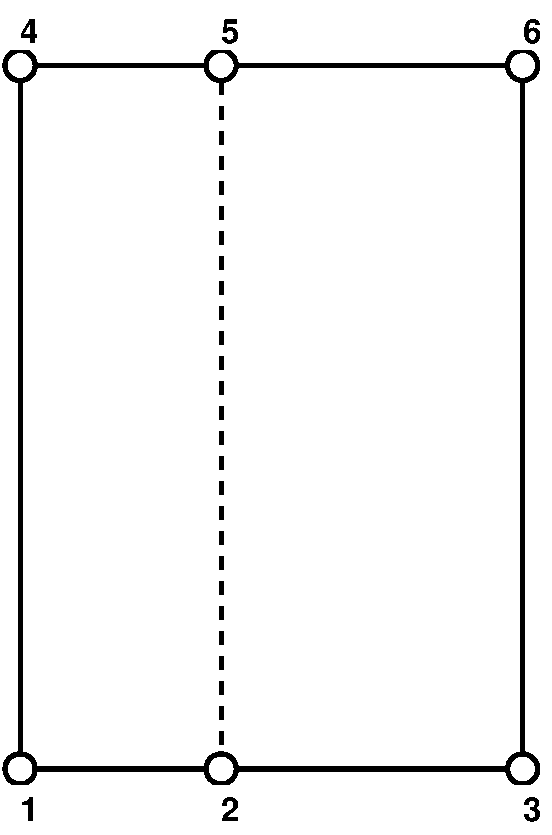
\includegraphics[height=3in]{figs/nblock2d}

\caption{Two dimensional NURBS surface patch \label{fig2b} }
\end{center}
\end{figure}

\begin{quote}
\noindent
\textbf{Example: 1-d NURBS Patch}

As an example consider again the parabola shown in Fig. \ref{fig1l}(a). The input
data using \texttt{NPATch} becomes:
\begin{verbatim}
       NURBs
         1  0 -12.0   0.0  1.0
         2  0   0.0  18.0  1.0
         3  0  12.0   0.0  1.0

       KNOTs
         open 1 6 0.0 0.0 0.0 1.0 1.0 1.0

       NPATch
         SURFace 1 3 1
           1  2  3

\end{verbatim}
\end{quote}

\subsubsection{\ul{Surface patch}}
           
Surface patches may be used to define either a two dimensional solids problem
or a three dimensional shell surface.
The surface patch of NURBS is specified using the command statements
\begin{verbatim}
       NPATch
         SURFace ma np1 np2 kn1 kn2
           cp(1,1) cp(2,1) .... cp(np1,1)
           cp(1,2) cp(2,2) .... cp(np1,2)
              ....
           cp(1,np2) ...........cp(np1,np2)
\end{verbatim}
In the above \texttt{ma} is the material number for the patch; \texttt{np1, np2}the number of control points along the two sides of the mesh;
\texttt{kn1, kn2} the knot
vectors in the two directions of the patch; and \texttt{cp(i,j)} are the 
NURBS control point numbers in which '\texttt{i}' is in the 1-direction
and '\texttt{j}' is in the 2-direction.

\begin{quote}
\noindent
\textbf{Example: 2-d NURBS Patch}

As an example consider again the patch shown in Fig. \ref{fig2b}. The input
form using the \texttt{NPATch} option becomes:
\begin{verbatim}
       NURBs
         1  0   0.0   0.0  1.0
         2  0  40.0   0.0  1.0
         3  0 100.0   0.0  1.0
         4  0   0.0 140.0  1.0
         5  0  40.0 140.0  1.0
         6  0 100.0 140.0  1.0

       KNOTs
         open 1 4 0.0 0.0 1.0 1.0
         open 2 5 0.0 0.0 0.5 1.0 1.0

       NPATch
         SURFace 1 2 3 1 2
           1  4
           2  5
           3  6
\end{verbatim}
\end{quote}

\subsubsection{\ul{Solid patch}}

\begin{figure}[b!]
\begin{center}

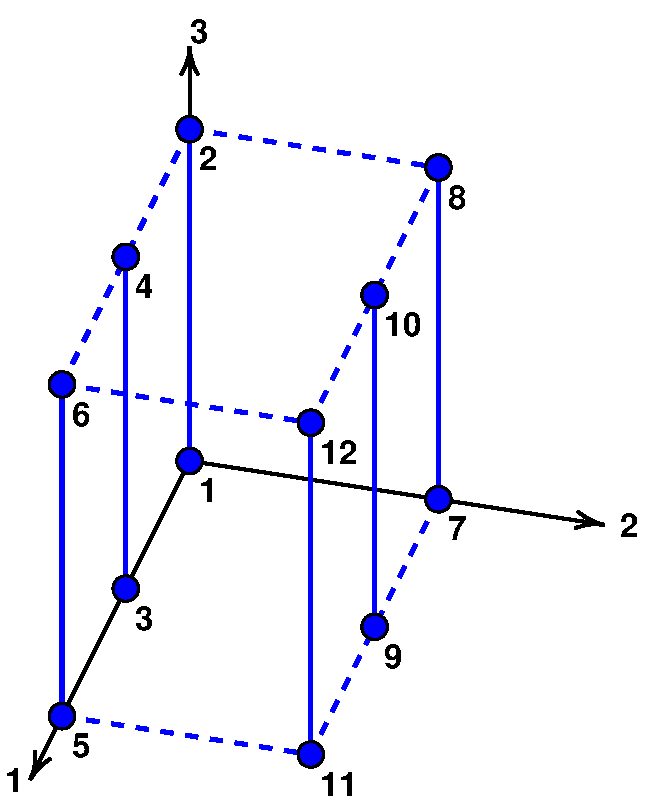
\includegraphics[height=3in]{figs/nblock3d}

\caption{Three dimensional NURBS solid patch \label{fig3b} }
\end{center}
\end{figure}

A three dimensional solid patch may be defined using the commands

\begin{minipage}{\textwidth}
\begin{verbatim}
       NPATch
         SOLId ma np1 np2 np3 kn1 kn2 kn3
           cp(1,1) cp(2,1) .... cp(np3,1)
           cp(1,2) cp(2,2) .... cp(np3,2)
              ....
           cp(1,np1) ...........cp(np3,np1)
           cp(1,np1+1) .........cp(np3,np1+1)
              ....
           cp(1,2*np1) .........cp(np3,2*np1)
           cp(1,2*np1+1) .......cp(np3,2*np1+1)
              ....
           cp(1,3*np1) .........cp(np3,3*np1)
           cp(1,3*np1+1) .......cp(np3,3*np1+1)
              ....
              ....
           cp(1,np1*np2) .......cp(np3,np1*np2)
\end{verbatim}
\end{minipage}

Where \texttt{ma} is the material number, \texttt{np1, np2, np3}, are the number of control points in the three directions of the block,
and \texttt{kn1, kn2, kn3} are the knot vector numbers in the three directions.

For a simple rectangular block the input data is given by

\begin{minipage}{\textwidth}
\begin{verbatim}
       NURBs
         1  0   0.0   0.0   0.0 1.0
         2  0   0.0   0.0  10.0 1.0
         3  0   5.0   0.0   0.0 1.0
         4  0   5.0   0.0  10.0 1.0
         5  0  10.0   0.0   0.0 1.0
         6  0  10.0   0.0  10.0 1.0
         7  0   0.0   6.0   0.0 1.0
         8  0   0.0   6.0  10.0 1.0
         9  0   5.0   6.0   0.0 1.0
        10  0   5.0   6.0  10.0 1.0
        11  0  10.0   6.0   0.0 1.0
        12  0  10.0   6.0  10.0 1.0

\end{verbatim}
\end{minipage}

\begin{minipage}{\textwidth}
\begin{verbatim}
       KNOTs
         open 1 6 0.0 0.0 0.0 1.0 1.0 1.0
         open 2 4 0.0 0.0 1.0 1.0
         open 3 4 0.0 0.0 1.0 1.0

       NPATch
         SOLId 1  3 2 2  1 2 3
           1  2
           3  4
           5  6
           7  8
           9 10
          11 12
\end{verbatim}
\end{minipage}

\subsection{Example: Two dimensional curved beam}

\begin{figure}[b!]
\begin{center}

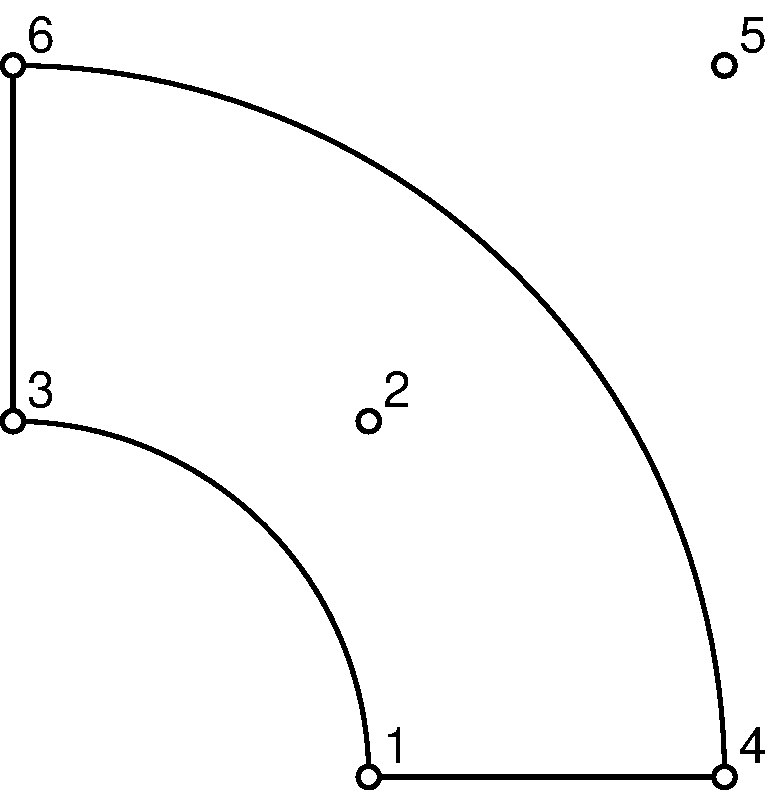
\includegraphics[width=3in]{figs/curve_mesh}

\caption{Curved beam mesh description. \label{fig2cb} }
\end{center}
\end{figure}

The complete data for a curved beam loaded by an end shear is given in
Table \ref{tab1} and shown in Fig.\ \ref{fig2cb}.

\begin{table}[!t]
\setlength{\baselineskip}{12pt}
\begin{verbatim}
       FEAP * * Curved beam NURBs solution
         0 0 0 2 2 0

       MATE
         solid
           elastic isotropic 1.e5 0.25
           nurb    interp      3    3

       EBOUndary
         1 0 1 0
         2 0 1 0

       EDISplacement
         2 0 0.1 0.0

       CBOUndary
         node 0 5 1 1

       KNOTs
         open 1 4 0.00 0.00 1.00 1.00
         open 2 6 0.00 0.00 0.00 1.00 1.00 1.00

       NURBs
         1 0  5.0  0.0  1.00
         2 0  5.0  5.0  1/sqrt(2)
         3 0  0.0  5.0  1.00
         4 0 10.0  0.0  1.00
         5 0 10.0 10.0  1/sqrt(2)
         6 0  0.0 10.0  1.00
          
       NPATch
         SURFace 1  3 2  2 1 
           1 2 3
           4 5 6

       END
\end{verbatim}
\setlength{\baselineskip}{14pt}
\caption{Input data for 2-d curved beam. \label{tab1}}
\end{table}
